    \documentclass[twocolumn,
        usenames, % allows access to some tikz colors
        dvipsnames % more colors: https://en.wikibooks.org/wiki/LaTeX/Colors
    ]{revtex4-1}% chktex 8
    \usepackage{
        amsmath,
        amssymb,
        fancyhdr, % page styling
        lastpage, % footer fanciness
        hyperref, % various links
        setspace, % line spacing
        amsthm, % newtheorem and proof environment
        mathtools, % \Aboxed for boxing inside aligns, among others
        float, % Allow [H] figure env alignment
        enumerate, % Allow custom enumerate numbering
        graphicx, % allow includegraphics with more filetypes
        wasysym, % \smiley!
        upgreek, % \upmu for \mum macro
        listings, % writing TrueType fonts and including code prettily
        tikz, % drawing things
        booktabs, % \bottomrule instead of hline apparently
        cancel % can cancel things out!
    }
    \usepackage[
        labelfont=bf, % caption names are labeled in bold
        font=scriptsize % smaller font for captions
    ]{caption}
    \usepackage[font=scriptsize]{subcaption} % subfigures

    \newcommand*{\scinot}[2]{#1\times10^{#2}}
    \newcommand*{\dotp}[2]{\left<#1\,\middle|\,#2\right>}
    \newcommand*{\rd}[2]{\frac{\mathrm{d}#1}{\mathrm{d}#2}}
    \newcommand*{\pd}[2]{\frac{\partial#1}{\partial#2}}
    \newcommand*{\rtd}[2]{\frac{\mathrm{d}^2#1}{\mathrm{d}#2^2}}
    \newcommand*{\ptd}[2]{\frac{\partial^2 #1}{\partial#2^2}}
    \newcommand*{\md}[2]{\frac{\mathrm{D}#1}{\mathrm{D}#2}}
    \newcommand*{\pvec}[1]{\vec{#1}^{\,\prime}}
    \newcommand*{\svec}[1]{\vec{#1}\;\!}
    \newcommand*{\ang}[0]{\;\text{\AA}}
    \newcommand*{\mum}[0]{\;\upmu \mathrm{m}}
    \newcommand*{\at}[1]{\left.#1\right|}

    \newtheorem{theorem}{Theorem}[section]

    \let\Re\undefined
    \let\Im\undefined
    \DeclareMathOperator{\Res}{Res}
    \DeclareMathOperator{\Re}{Re}
    \DeclareMathOperator{\Im}{Im}
    \DeclareMathOperator{\Log}{Log}
    \DeclareMathOperator{\Arg}{Arg}
    \DeclareMathOperator{\Tr}{Tr}
    \DeclareMathOperator{\E}{E}
    \DeclareMathOperator{\Var}{Var}
    \DeclareMathOperator*{\argmin}{argmin}
    \DeclareMathOperator*{\argmax}{argmax}
    \DeclareMathOperator{\sgn}{sgn}
    \DeclareMathOperator{\diag}{diag\;}

    \DeclarePairedDelimiter\bra{\langle}{\rvert}
    \DeclarePairedDelimiter\ket{\lvert}{\rangle}
    \DeclarePairedDelimiter\abs{\lvert}{\rvert}
    \DeclarePairedDelimiter\ev{\langle}{\rangle}
    \DeclarePairedDelimiter\p{\lparen}{\rparen}
    \DeclarePairedDelimiter\s{\lbrack}{\rbrack}
    \DeclarePairedDelimiter\z{\lbrace}{\rbrace}

    % \everymath{\displaystyle} % biggify limits of inline sums and integrals
    \tikzstyle{circ} % usage: \node[circ, placement] (label) {text};
        = [draw, circle, fill=white, node distance=3cm, minimum height=2em]
    \definecolor{commentgreen}{rgb}{0,0.6,0}
    \lstset{
        basicstyle=\ttfamily\footnotesize,
        frame=single,
        numbers=left,
        showstringspaces=false,
        keywordstyle=\color{blue},
        stringstyle=\color{purple},
        commentstyle=\color{commentgreen},
        morecomment=[l][\color{magenta}]{\#}
    }

\begin{document}

\def\Snospace~{\S{}} % hack to remove the space left after autorefs
\renewcommand*{\sectionautorefname}{\Snospace}
\renewcommand*{\appendixautorefname}{\Snospace}
\renewcommand*{\figureautorefname}{Fig.}
\renewcommand*{\equationautorefname}{Eq.}
\renewcommand*{\tableautorefname}{Tab.}

\title{IGWs and WDs Ongoing Writeup}
\author{Yubo Su}
\maketitle

\section{Introduction}

WIP ongoing writeup, last updated \today.

% Define white dwarfs (WD), internal gravity waves (IGW), citations

Basic narrative is: the prevailing understanding is that mean flow absorption
slowly spins up a WD from the outside in as the critical layer propagates
inwards. Our numerical simulations validate this prediction and give an
analytical prediction for the motion of the critical layer. However, it appears
our numerical simulations are viscosity limited. We present a brief argument for
why the viscosity limitations are insignificant, but also present some
exploratory, inconclusive work towards direct numerical simulation resolving
critical layer behavior without being viscosity limited.

In \autoref{s:eq}, we will cover the equations and numerical setup. In
\autoref{s:lin}, we will discuss the agreement of our simulation in the
low-amplitude limit with analytical linear theory. In \autoref{s:nonlin} we will
present a few reference simulations illustrating critical layer absorption
depositing horizontal angular momentum into the fluid. Finally, in
\autoref{s:bouss} we will consider a speculative series of simulations
attempting to rectify the seemingly viscosity-limited simulations of the
previous section.

\section{Equations}\label{s:eq}

We simulate an incompressible, isothermal fluid, representatitive of degenerate
matter in WD bulks. We assume a barotropic equation of state as a first
approximation. Furthermore, we model the background, hydrostatic density
stratification as $\rho_0(x, z) = \rho_0(z) \propto e^{-z/H}$.

The physical equations for an incompressible, barotropic fluid in a uniform
gravitational field are
\begin{subequations}\label{se:fc_orig}
    \begin{align}
        \vec{\nabla} \cdot \vec{u} &= 0,\\
        \pd{\rho}{t} + \vec{u} \cdot \vec{\nabla}\rho &= 0
            ,\label{eq:fc_density}\\
        \pd{\vec{u}}{t} + \p*{\vec{u} \cdot \vec{\nabla}}\vec{u}
            + \frac{\vec{\nabla}P}{\rho}
            + g\hat{z} &= 0.
    \end{align}
\end{subequations}
$\vec{u}, \rho, P$ are the fluid dynamical variables and $-g\hat{z}$ is constant
gravitational acceleration. Note that at hydrostatic equilibrium $\partial_t =
0$ we have $\vec{u} = 0, \vec{\nabla}P_0 = -\rho_0 g\hat{z}$ and so $P_0 =
\rho_0 gH$.

We nondimensionalize by taking $H = N = \rho_{ref} = 1$ where
\begin{equation}
    N^2 \equiv g^2\p*{\rd{\rho}{P} - \at{\pd{\rho}{P}}_{ad}}
        = \frac{g}{H},
\end{equation}
is the Brunt-V\"ais\"al\"a frequency and $\rho_{ref}$ is the background density
stratification at $z = 0$. The full numerical details of the simulation are
described in \autoref{ss:strat_impl}.

\subsection{Wave Generation}

To model a continuous IGW wave train excited deep in the WD interior propagating
towards the surface without unnecessary computational cost, we excite an
IGW wave train from the bottom of the simulation domain. As Chebyshev grid is
a factor of $\propto N_z$ denser near the edges of the simulation domain, we
use a volumetric forcing to excite IGW at some $z_0 > 0$ interior to the
simulation domain. Our forcing excites both IGW propagating upwards, the
physically interesting solution, and downwards, which are damped away by damping
layers (see \autoref{ss:strat_impl}) before inducing strict Courant-Friedrichs-Lewy
(CFL) timestepping constraints (cite).

As not to interfere with the incompressibility constraint, we force the system
on the density equation, replacing \autoref{eq:fc_density} with
\begin{equation}
    \pd{\rho}{t} + \vec{u} \cdot \vec{\nabla}\rho =
        Fe^{-\frac{(z - z_0)^2}{2\sigma^2}}
            \cos \p*{k_{0, x}x - \omega_0 t}.
\end{equation}
Define $k_{0, z}: \omega(k_{0, x}, k_{0, z}) = \omega_0$. If $k_{0, z}\sigma \ll
1$, the forcing term has the effect of picking out $k_{0, z}$ driven by
$\cos\p*{k_{0, x}x - \omega_0 t}$ from the broad $k_z$ wavenumber spectrum
permitted by the narrow Gaussian profile.

\section{Linear Regime}\label{s:lin}

We first test our numerical simulation with a ``linear'' simulation, where
all flow quantities are small: we assume  $\rho_1 \equiv \rho - \rho_0 \ll
\rho_0$ and $\vec{u} \cdot \vec{\nabla} \ll \partial_t$. We clarify that our
``linear'' simulations solve the full nonlinear equations, just in the weak
perturbation limit.

\subsection{Analytical Solution}

In the small perturbation limit, we linearize \autoref{se:fc_orig} with
inhomegeneous driving term and obtain:
\begin{subequations}\label{se:vol_drive}
    \begin{align}
        \vec{\nabla} \cdot \vec{u} &= 0,\\
        \pd{\vec{u}_1}{t} + \frac{\vec{\nabla}P}{\rho_0}
            + \frac{\rho_1 \vec{g}}{\rho_0}
            &= 0,\\
        \pd{\rho_1}{t} - \frac{u_{1z} \rho_0}{H}
            &= Fe^{-\frac{(z - z_0)^2}{2\sigma^2}}
                e^{i(k_xx - \omega t)}.
    \end{align}
\end{subequations}
We have substituted $\cos\p*{k_xx - \omega_0t}$ for a complex exponential for
easier manipulation; taking real parts of all dynamical variables above recovers
the physical solution.

It is well known that the solutions to the $F = 0$ homogeneous
\autoref{se:vol_drive} are of form (cite)
\begin{subequations}\label{se:lin_sol}
    \begin{align}
        u_z\p*{x, z, t} &= Ae^{z/2H}e^{i(k_{0x}x + k_{0z}z - \omega_0 t)},\\
        \omega_0^2 &= \frac{N^2k_{0x}^2}{k_{0x}^2 + k_{0z}^2 + \frac{1}{4H^2}}.
    \end{align}
\end{subequations}

To solve the inhomogeneous system, we may first approximate the driving term
using $e^{\frac{-(z - z_0)^2}{2\sigma^2}} \approx \sqrt{2\pi \sigma^2}\delta(z -
z_0)$ if $\sigma \to 0$, then relax to $k_{0z}\sigma \lesssim 1$. This may be
solved to obtain the solution
\begin{align}
    A(F) &= \frac{Fgk_{0x}^2}{\rho_0(z_0)\omega_0^2}
        \frac{1}{2ik_z}\frac{e^{\frac{-(k_{0z}\sigma)^2}{2}}}
        {\sqrt{2\pi\sigma^2}},\\
    u_{1z} &= A(F) \times\begin{cases}
        e^{\frac{z - z_0}{2H}}e^{i(k_{0x}x + k_{0z}(z - z_0) - \omega_0 t)}
            & z > z_0\\
        e^{\frac{z - z_0}{2H}}e^{i(k_{0x}x - k_{0z}(z - z_0) - \omega_0 t)}
            & z < z_0\\
    \end{cases}.\label{eq:uz_lin}
\end{align}
The extra factor of $e^{-\frac{(k_{0z}\sigma)^2}{2}}$ compared to the
$\delta$-function solution comes from evaluating the Fourier Transform of
$e^{-\frac{(z - z_0)^2}{2\sigma^2}}$ at $k_z = k_{0z}$.

Furthermore, in the low-amplitude, dissipation free limit, the time-averaged
total $x$-momentum flux in the $\hat{z}$ direction can be computed. Since all
dynamical variables $\propto e^{i(k_{0x}x - \omega_0 t)}$, $x$ averaging and
time averaging are equivalent, so we may write
\begin{equation}
    F_{px} \equiv \frac{1}{L_x}\int_0^{L_x}\limits \rho u_x u_z\;\mathrm{d}x
\end{equation}
We will denote this $F_{px} = \ev*{\rho u_xu_z}_x$ for simplicity. For a given
forcing amplitude then:
\begin{equation}
    F_{px}(F) \approx -\frac{A(F)^2}{2}\rho_0(z_0) \frac{k_z}{k_x}.
        \label{eq:fpx_lin}
\end{equation}
We've approximated $k_zH \ll 1$ and noticed $\ev*{\rho_1 u_xu_z}_x = 0$ in the
above for clarity.

Finally, it may be noted that horizontally averaged horizontal momentum
$p_x = \ev*{\rho u_x}_x$ obeys $\pd{p_x}{t} + \pd{F_{px}}{z} = 0$, and since
flux is transported on the group velocity timescale, this simplifies to the
known expression for the wave-induced horizontal mean flow (cite)
\begin{equation}
    \bar{U}_0 \equiv \ev*{u_x}_x = \frac{\ev*{u_xu_z}_x}{c_{gz}}
\end{equation}
We've denoted $c_{gz} = \at{\pd{\omega}{k_{z}}}_{k_{z0}}$ the vertical group
velocity. In terms of our forcing amplitude,
\begin{equation}
    \bar{U}_0(F) = -\frac{A(F)^2}{2}e^{\frac{z - z_0}{H}} \frac{k_z}{k_x}c_{gz},
        \label{eq:u0_lin}
\end{equation}
where $c_{gz} = -\frac{Nk_{0x}k_{0z}}{\p*{k_{0x}^2 + k_{0z}^2 +
\frac{1}{4H^2}}^{3/2}}$.

$\omega$ is chosen by inverting $\omega(k_x, k_z)$ dispersion relation for fixed
$k_x = 2\pi / L_x$ and some desired $k_z = -2\pi/H$, and $\sigma \lesssim
\frac{1}{k_z}$ is used to excite a broad band of modes including the desired
$k_z$ mode.

\subsection{Numerical Simulation}\label{ss:lin_ns}

We simulate using Dedalus (cite) a spectral numerical method. We use a Fourier
basis in the $x$ direction and a Chebyshev in the $z$ direction. Our simulation
starts with all perturbation quantities at zero, an initial condition at rest.
Our parameters are chosen to be as similar as possible to the later nonlinear
simulations (\autoref{s:nonlin}). We choose as follows:
\begin{itemize}
    \item $k_{0x}$: Astrophysical IGWs have $k_x \ll k_z$, so we choose $k_{0x}
        = \frac{2\pi}{L_x}$ the smallest permitted wavenumber permitted by
        periodic boundary conditions.

    \item We choose $\omega_0$ by choosing it to produce a desired $k_{0z}$.
        Astrophysical systems generally also exhibit $k_zH \gg 1$, where the
        stratification height is significantly larger than the vertical
        wavelength. However, in order for the simulation to both be well-damped
        at grid resolutions and be neglibily damped at leading order nonlinear
        wavelengths, we require $k_{0z} \ll \frac{1}{L_{NL}} \ll \frac{2\pi
        N_z}{L_z}$, where $L_{NL}$ denotes some characteristic length scale of
        nonlinear features. Finally, we need $L_z$ to be many $H$ to capture
        significant $e^{z/2H}$ growth and separate the linear and nonlinear
        amplitudes of $u_z$.

        Fixing $L_z = 10H$ to give $\sim e^4$ amplitude growth between the
        damping zones, this implies we require separation of scales $1 \ll
        k_{0z}H \ll \frac{H}{L_{NL}} \ll \frac{2\pi N_z}{10}$.

        Since $N_z$ is fixed by computational cost (we tried both $N_z = 512,
        N_z = 1024$), we choose $k_{0z} \sim \frac{2\pi}{H}$. This is less
        physically representative but gives more wavenumber space for the
        nonlinear cascade. We then invert $\omega_0 = \omega(k_{0x}, k_{0z})$.

    \item We choose $\nu$ $1/10$ that of the nonlinear simulation, to verify
        that the undamped linear solution is recovered.

    \item We choose $F$ forcing strength $1/20$ that of the nonlinear
        simulation, which keeps the flow amplitude sufficiently small to be
        treated in the linear approximation at all points in the simulation
        domain.
\end{itemize}

A representative snapshot of this simulation
is provided in \autoref{fig:linear_nonu}. Key features to note:
\begin{itemize}
    \item $u_z$ grows with \autoref{eq:uz_lin} to reasonable accuracy.

    \item $F_{px}$ is seen to be constant, as would be expected by
        \autoref{eq:fpx_lin}.

    \item $\bar{U}_0$ agrees with \autoref{eq:u0_lin} at lower $z$ but deviates
        significantly at higher $z$. This deviation is caused by the top damping
        zone that does not conserve horizontal momentum.
\end{itemize}
We also include a qualitatively similar snapshot of the same simulation run
using the $\nu$ from the later nonlinear simulations in \autoref{fig:linear_nu}.
\begin{figure}[h]
    \centering
    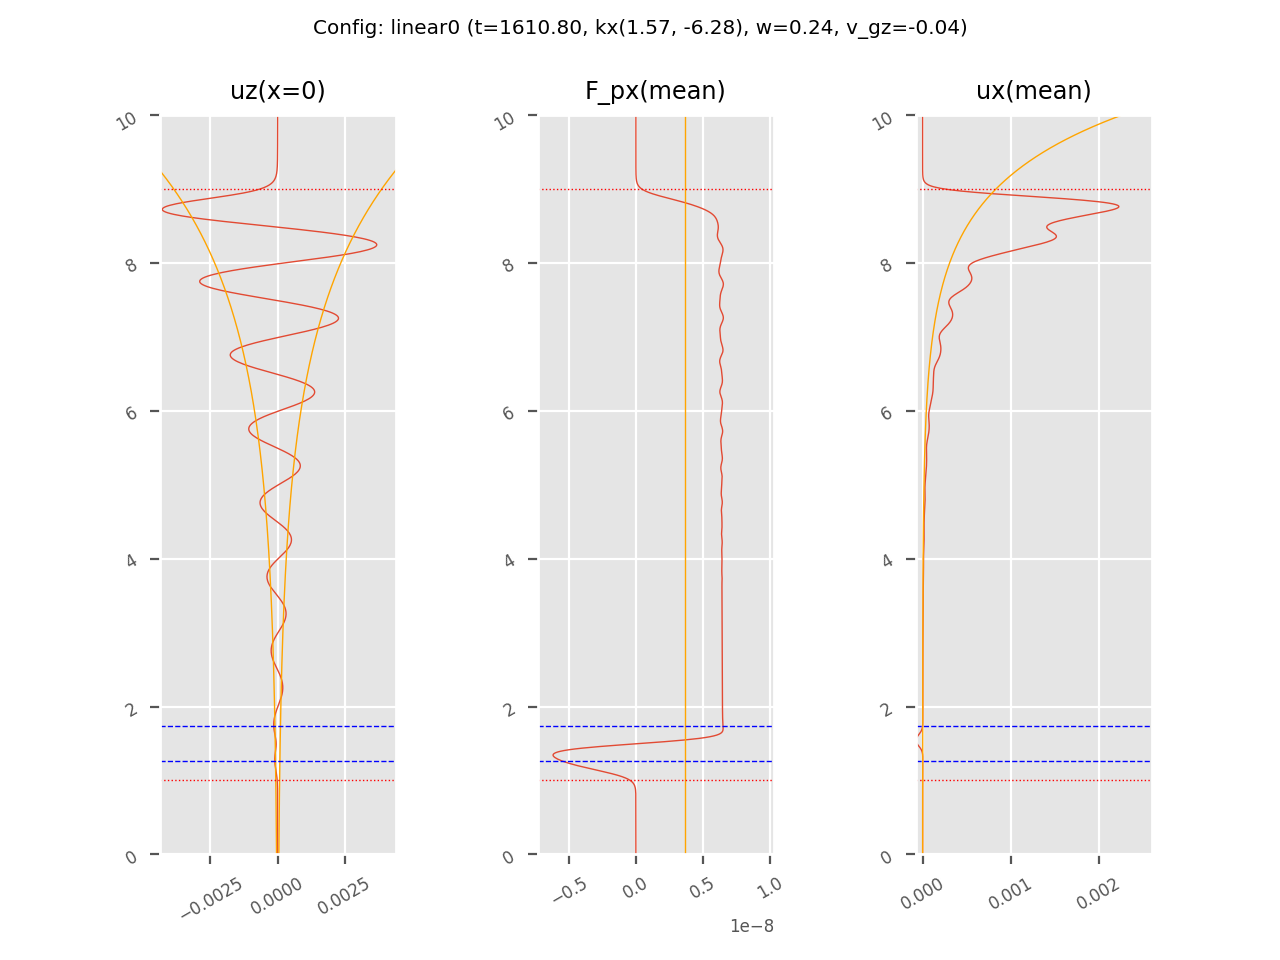
\includegraphics[width=0.5\textwidth]{plots/linear_nonu.png}
    \caption{Snapshot of linear simulation after reaching steady state.
        Analytical predictions of $\abs*{u_z}, \bar{U}_0, F_{px}$ are shown in
        orange. Red dotted lines indicate the onset of the damping region and
        blue dotted lines denote the driving region.}\label{fig:linear_nonu}
\end{figure}
\begin{figure}[h]
    \centering
    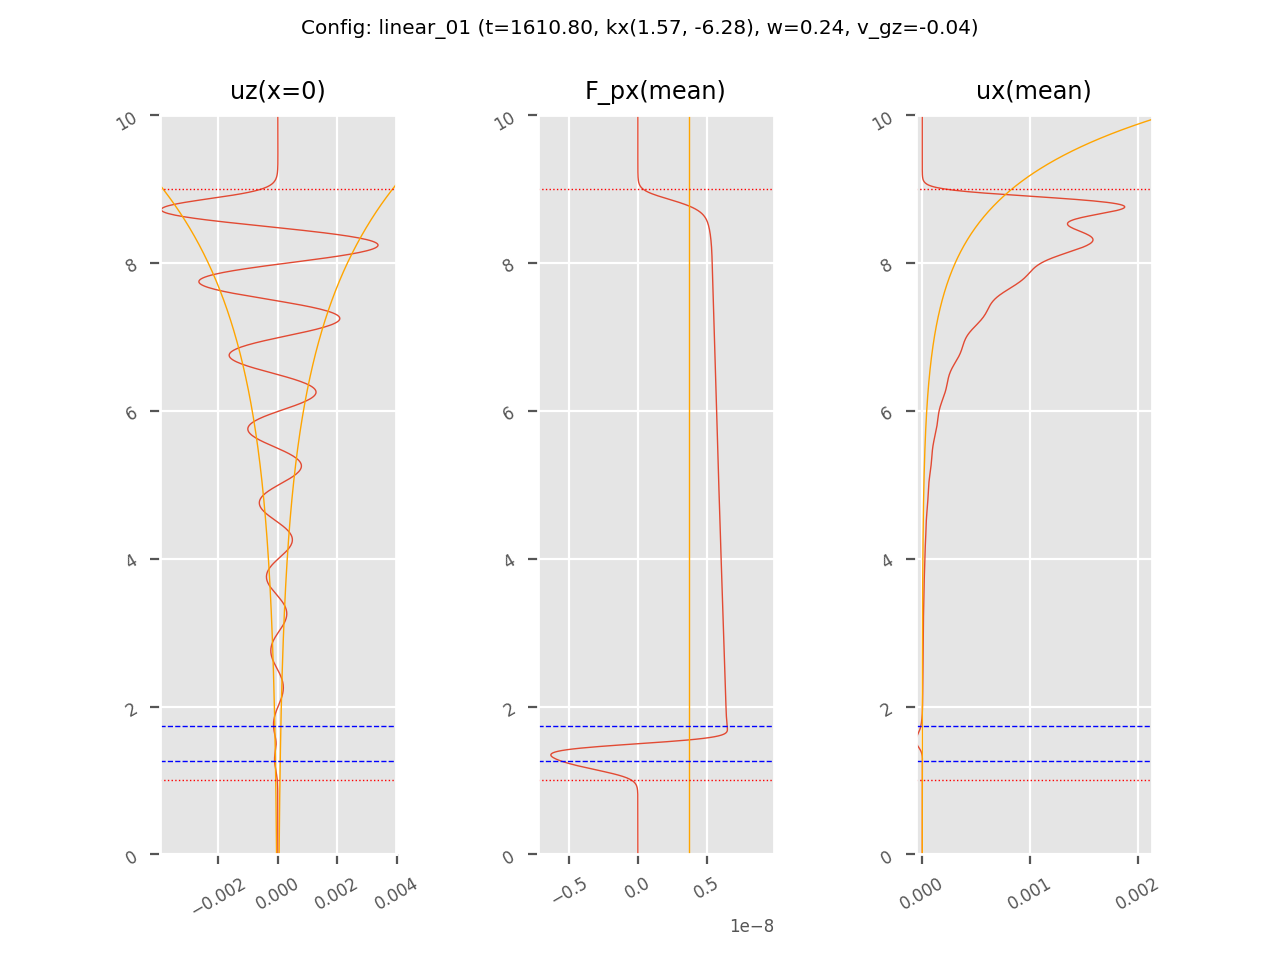
\includegraphics[width=0.5\textwidth]{plots/linear_nu.png}
    \caption{Same as \autoref{fig:linear_nonu} but with $0.3\times $viscosity
    used for nonlinear simulations (YUBONOTE should be the same but that
    simulation mysteriously stopped without me noticing; restarting worked, so
    currently rerunning). Note the slight resulting dissipation in $F_{px}$.
    }\label{fig:linear_nu}
\end{figure}

\section{Nonlinear Regime}\label{s:nonlin}

\subsection{Mean Flow Critical Layer Absorption}

In past studies of IGWs in WDs (cite Fuller \& Lai), $\xi_z \equiv
\frac{u_z}{\omega_0}$ the Lagrangian fluid displacement was often used towards
wave breaking criterion $k_{0z}\xi_z \gtrsim 1$. We argue that the wave's
self-interaction via its generated mean flow $\bar{U}_0$ induces total
absorption when the mean flow exceeds critical value
\begin{equation}
    \bar{U}_c = \frac{\omega_0}{k_{0x}}.
\end{equation}
This is consistent with the picture put forth in e.g.\ Goldreich and Nicholson
(cite).

A purely horizontal shear flow $\bar{U}_0(z) \hat{x}$ can be seen in
\autoref{se:fc_orig} to have the effect of modifying time derivatives
$\partial_t$ to their frequency in the comoving frame of the fluid $\partial_t -
\bar{U}_0(z)\partial_x$. For a critical value $\omega_0 - \bar{U}_c k_{0x} = 0$,
the frequency of the linear wave in the fluid's frame of reference vanishes and
critical behavior is observed. In a linear theory or a theory where small scales
are viscosity rather than advection dominated, the incident wave has amplitude
reflection and transmission coefficients
\begin{align}
    \mathcal{R} &= e^{-2\pi \sqrt{\mathrm{Ri} - \frac{1}{4}}}, &
    \mathcal{T} &= e^{-\pi \sqrt{\mathrm{Ri} - \frac{1}{4}}},
    \label{eq:crit_coeffs}
\end{align}
where we have defined Richardson number $\mathrm{Ri} \equiv
\at{\frac{N^2}{\p*{\pd{\bar{U}_0}{z}}^2}}_{z_c}$ at the critical layer $z_c:
\bar{U}_0(z_c) = \frac{\omega_0}{k_{0x}}$. For most shear flows, $\mathrm{Ri}
\gg 1$ and so $\mathcal{R}, \mathcal{T} \ll 1$ and the incident wave is
absorbed.

When the fluid absorbs the incident wave, it absorbs the incident horizontal
momentum flux as well, which is converted into additional horizontal momentum of
the shear flow. Since the shear flow cannot exceed $\bar{U}_c$ the horizontal
phase velocity of the incident wave, the critical layer must thus propagate
downwards (towards the wave source) to accommodate the incident momentum. In
other words, the total horizontal momentum of the shear flow obeys conservation
equation
\begin{equation}
    \pd{}{t}\int\limits_0^{L_z} \rho(z) \bar{U}_0(z, t)\;\mathrm{d}z
        - F_{px} = 0.
\end{equation}
Treating $\bar{U}_0(z > z_c) = \bar{U}_c, \bar{U}(z < z_c) = 0$ gives us exactly
\begin{equation}
    \rho \bar{U}_c\pd{z_c}{t} = -F_{px}.\label{eq:zc_anal}
\end{equation}

\subsection{Numerical Simulation}

We use the same $k_{0x}, \omega_0$ as \autoref{ss:lin_ns}. Our other parameters
are:
\begin{itemize}
    \item We choose $\nu = 0.35 \frac{\omega_0}{k_{0z}k_{z, \max}}$, where
        $k_{z, \max} = \frac{2\pi N_z}{L_z}$. Note that $\nu =
        \frac{\omega_0}{k_{0z} k_{z, \max}}$ corresponds to the advective term
        $\vec{u} \cdot \vec{\nabla}$ being of the same order as the time
        derivative $\partial_t$ for flow velocities $\vec{u} \sim
        \frac{\omega_0}{k_{0z}}$ at the grid spacing.

    \item We choose $F$ such that $\bar{U}_0(z)$ predicted by
        \autoref{eq:u0_lin} exceeds $\bar{U}_c$ critical velocity for $z <
        L_z$, i.e.\ the wave-induced mean flow is sufficiently large within the
        simulation domain to induce critical layer absorption.
\end{itemize}

Two representative snapshots from our simulation are provided in
\autoref{fig:nl} after the critical layer has had time to form. We may note that
the critical layer, where $F_{px}$ is absorbed and $\bar{U}_0 = \bar{U}_c$,
travels downwards as predicted.
\begin{figure}[h]
    \centering
    \begin{subfigure}{0.5\textwidth}
        \centering
        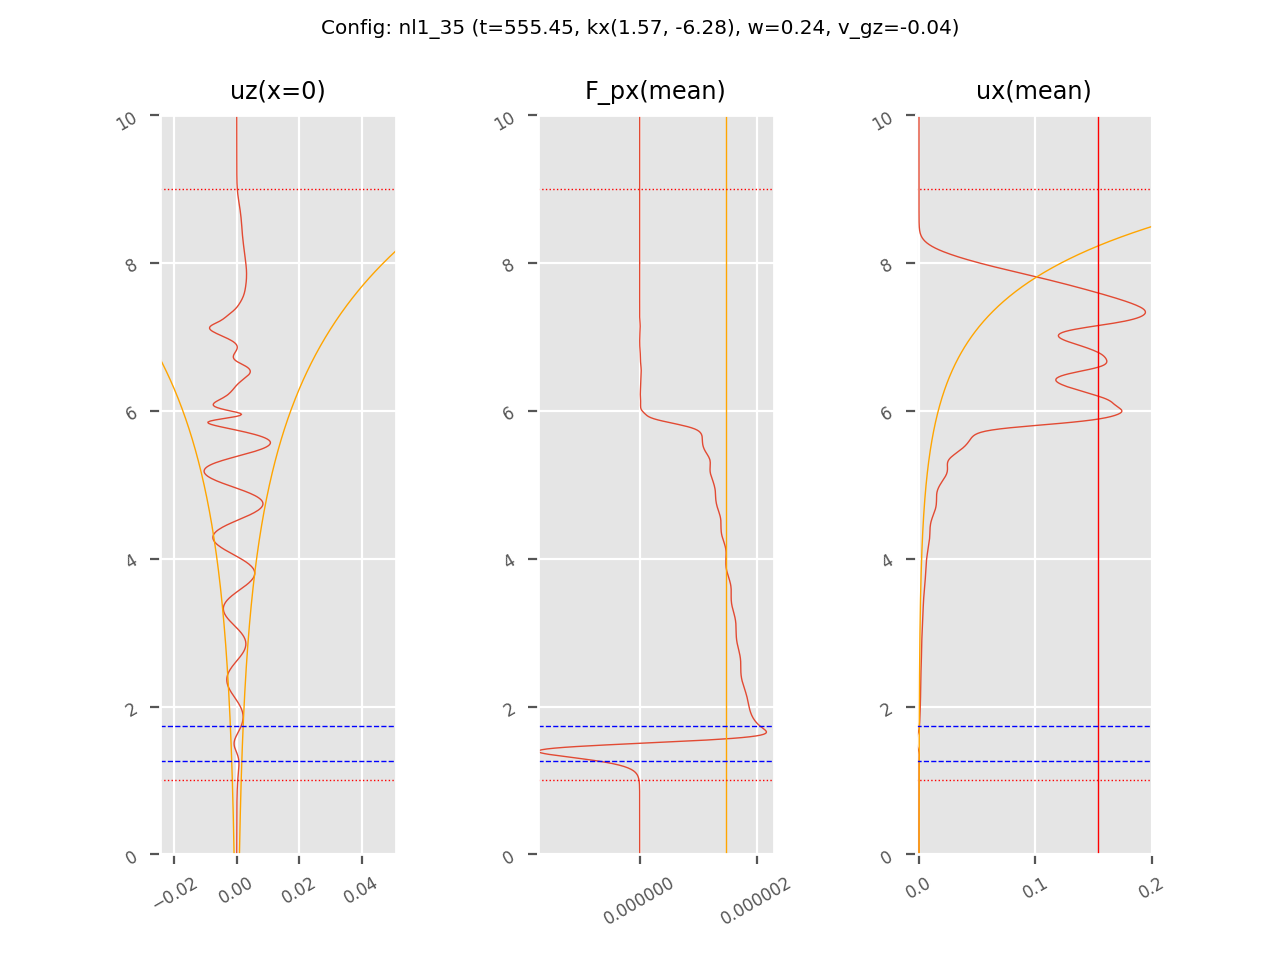
\includegraphics[width=\textwidth]{plots/nl35_1.png}
        \caption{Earlier time snapshot. Legend is the same as
        \autoref{fig:linear_nonu} except $\bar{U}_c$ is marked in red on the
        third panel.}
    \end{subfigure}

    \begin{subfigure}{0.5\textwidth}
        \centering
        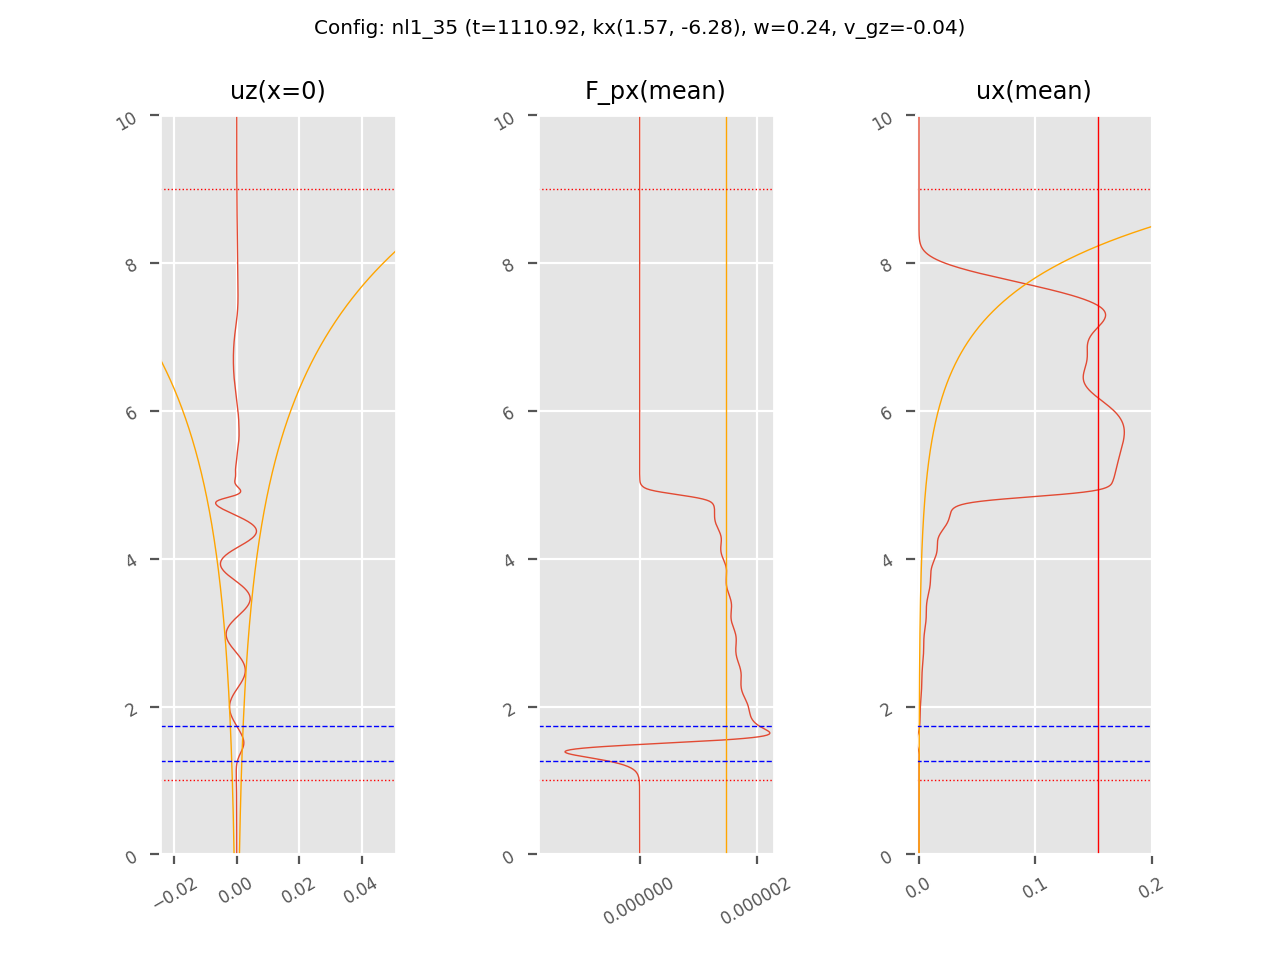
\includegraphics[width=\textwidth]{plots/nl35_2.png}
        \caption{Later snapshot illustrating propagation of $z_c$.}
    \end{subfigure}
    \caption{Nonlinear numerical simulation.}\label{fig:nl}
\end{figure}

\subsection{Propagating Critical Layer}

For the simulation in \autoref{fig:nl}, we may define $z_c = \argmax_z
\pd{\bar{U}_0}{z}$. Computing $\pd{z_c}{t}$ using the analytical flux
\autoref{eq:fpx_lin} allows comparison to \autoref{eq:zc_anal}, which we exhibit
in \autoref{fig:zc_anal}. We see overall good agreement, though some small
deviation is expected since $F_{px}$ is not perfectly conserved owing to
numerical viscosity (and YUBONOTE $F_{px}$ is misestimated?).
\begin{figure}[h]
    \centering
    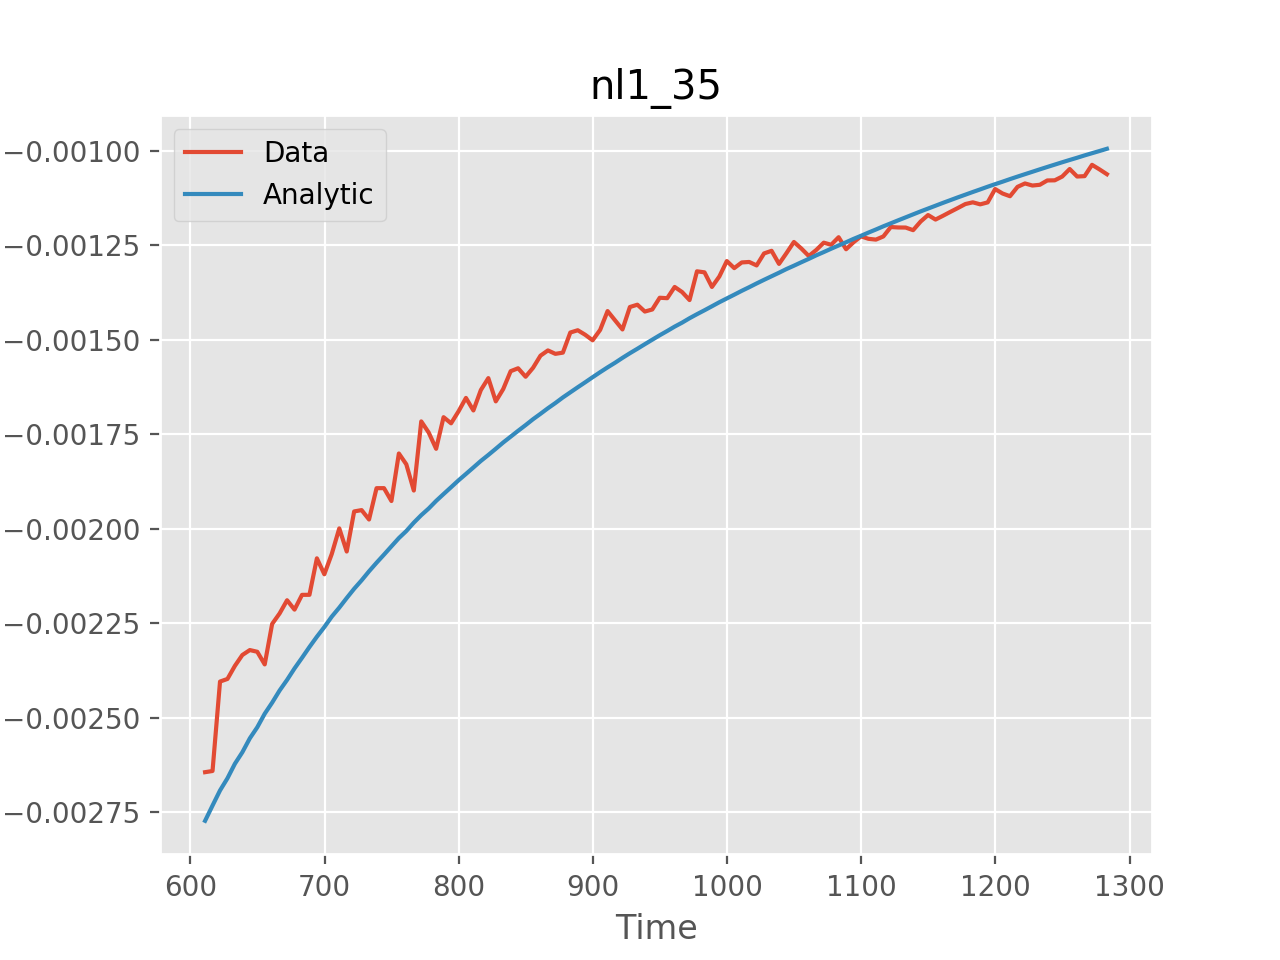
\includegraphics[width=0.5\textwidth]{plots/nl35_front_v.png}
    \caption{Comparison of simulated $\pd{z_c}{t}$ to analytical
    \autoref{eq:zc_anal}. Plot begins after formation of critical layer in
    simulation.}\label{fig:zc_anal}
\end{figure}

However, recalling \autoref{eq:crit_coeffs}, we only expect complete critical
layer absorption when $\mathrm{Ri} \gg \frac{1}{4}$. We may plot $\mathrm{Ri}$
over the same time interval in \autoref{fig:nl35_f_ri}. We may observe that the
Richardson number is initially decreasing but eventually levels out and
begins to increase again. This corresponds to an increasingly sharp critical
layer transition then subsequently a decreasingly sharp critical layer
transition.
\begin{figure}[h]
    \centering
    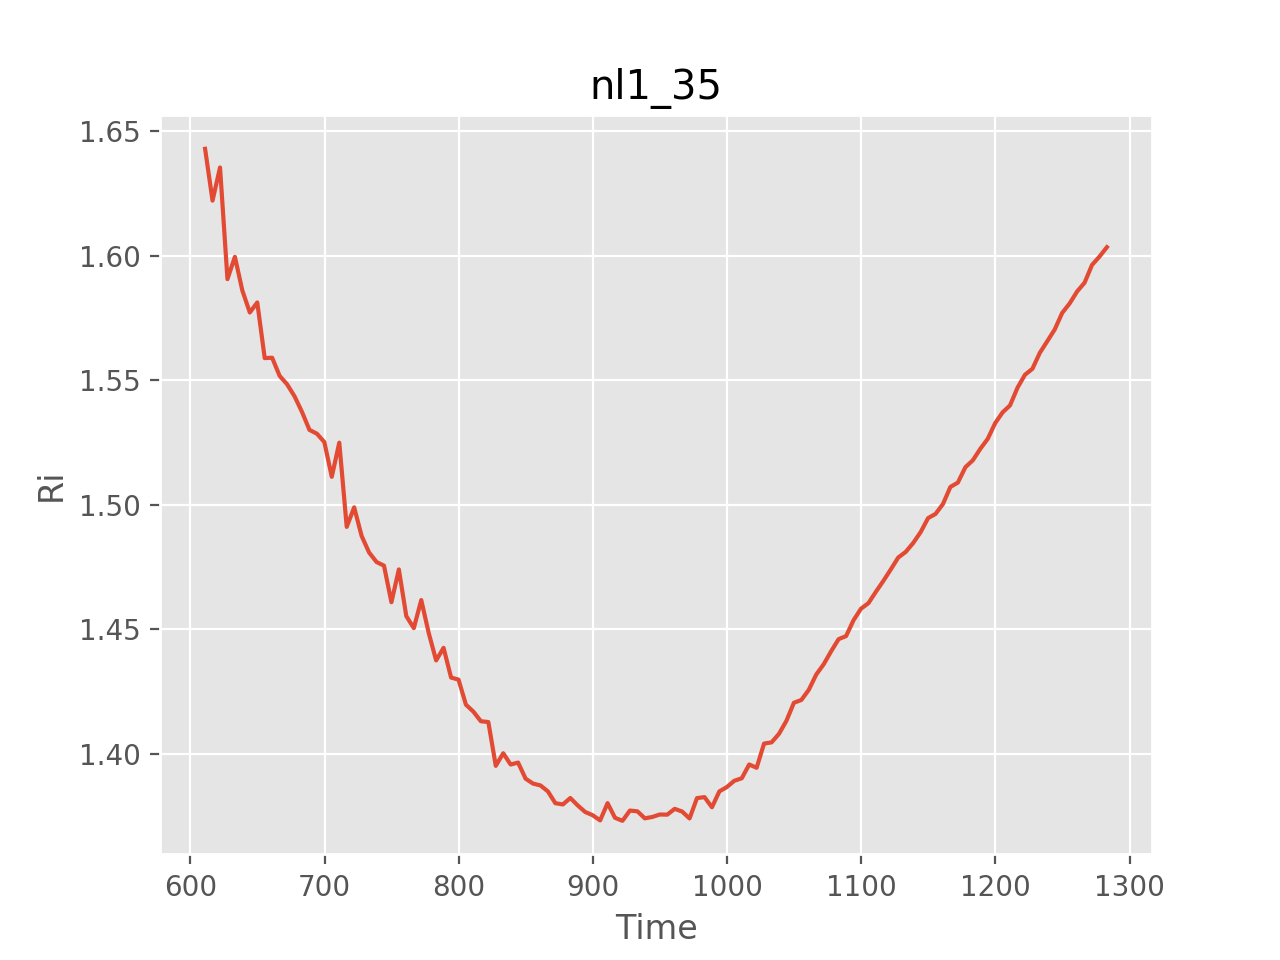
\includegraphics[width=0.5\textwidth]{plots/nl35_f_ri.png}
    \caption{Plot of $\mathrm{Ri}_{\max}(t) = \max_z
    \frac{N^2}{\bar{U}_0'}(t)$ over the simulation time.}\label{fig:nl35_f_ri}
\end{figure}

We argue that the Richardson number is bounded from below by viscosity. A
repeated simulation with a larger viscosity is shown in \autoref{fig:nl1_f_ri},
where the Richardson number does not go nearly as low.
\begin{figure}[h]
    \centering
    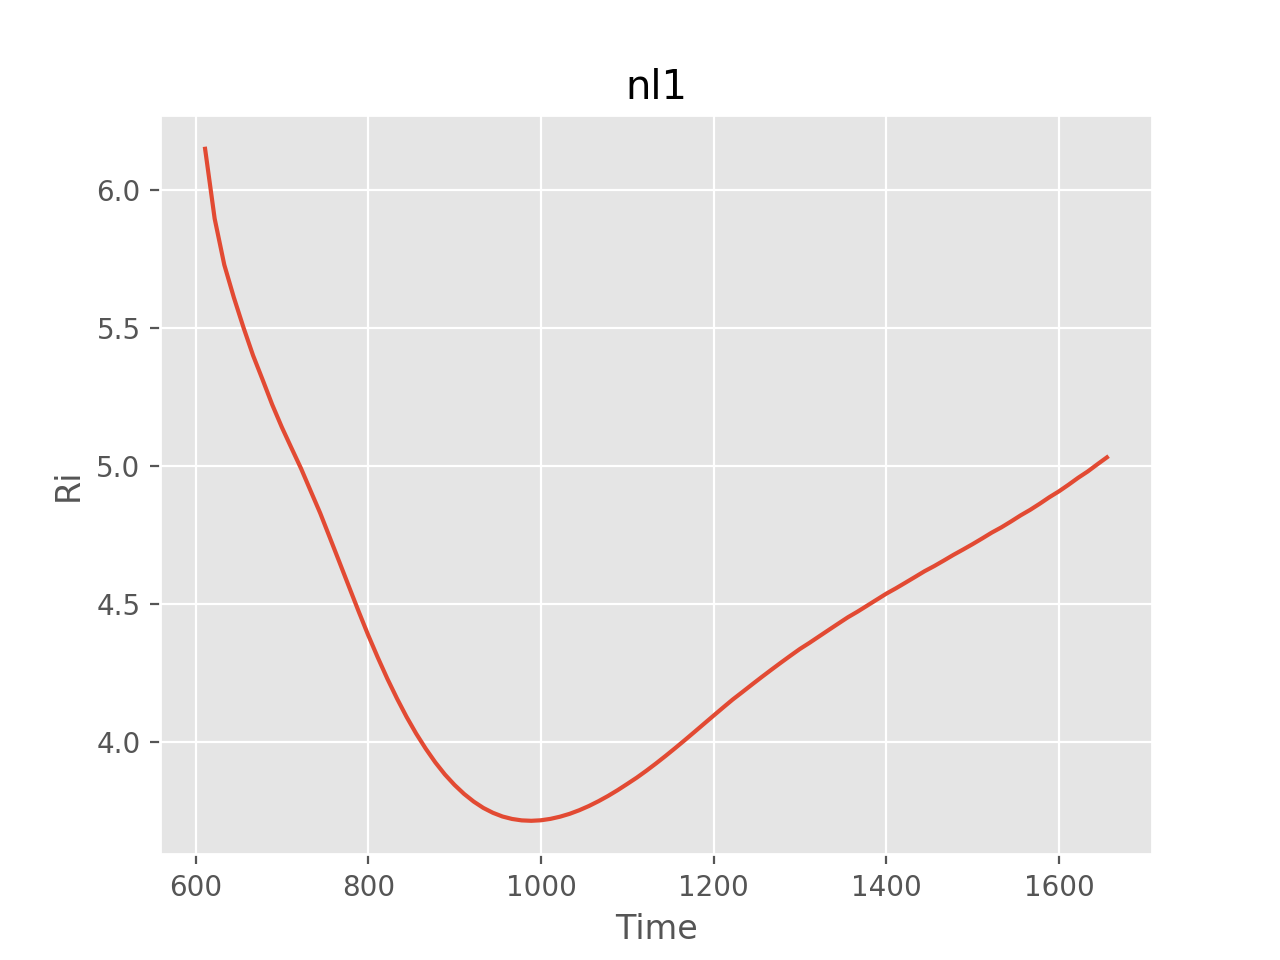
\includegraphics[width=0.5\textwidth]{plots/nl1_f_ri.png}
    \caption{Same as \autoref{fig:nl35_f_ri} but with $\sim 1.3\times$
    viscosity.}\label{fig:nl1_f_ri}
\end{figure}

Additionally, a lower-viscosity simulation shows significant features resembling
Kelvin-Helmholtz instabilities (KHI), \autoref{fig:nl_full_01}. As we have only
plotted $\bar{U}_0(z)$, the local Richardson number $N^2 / \pd{u_x}{z}$ may
exceed the plotted value and incur KHIs.
\begin{figure}[h]
    \centering
    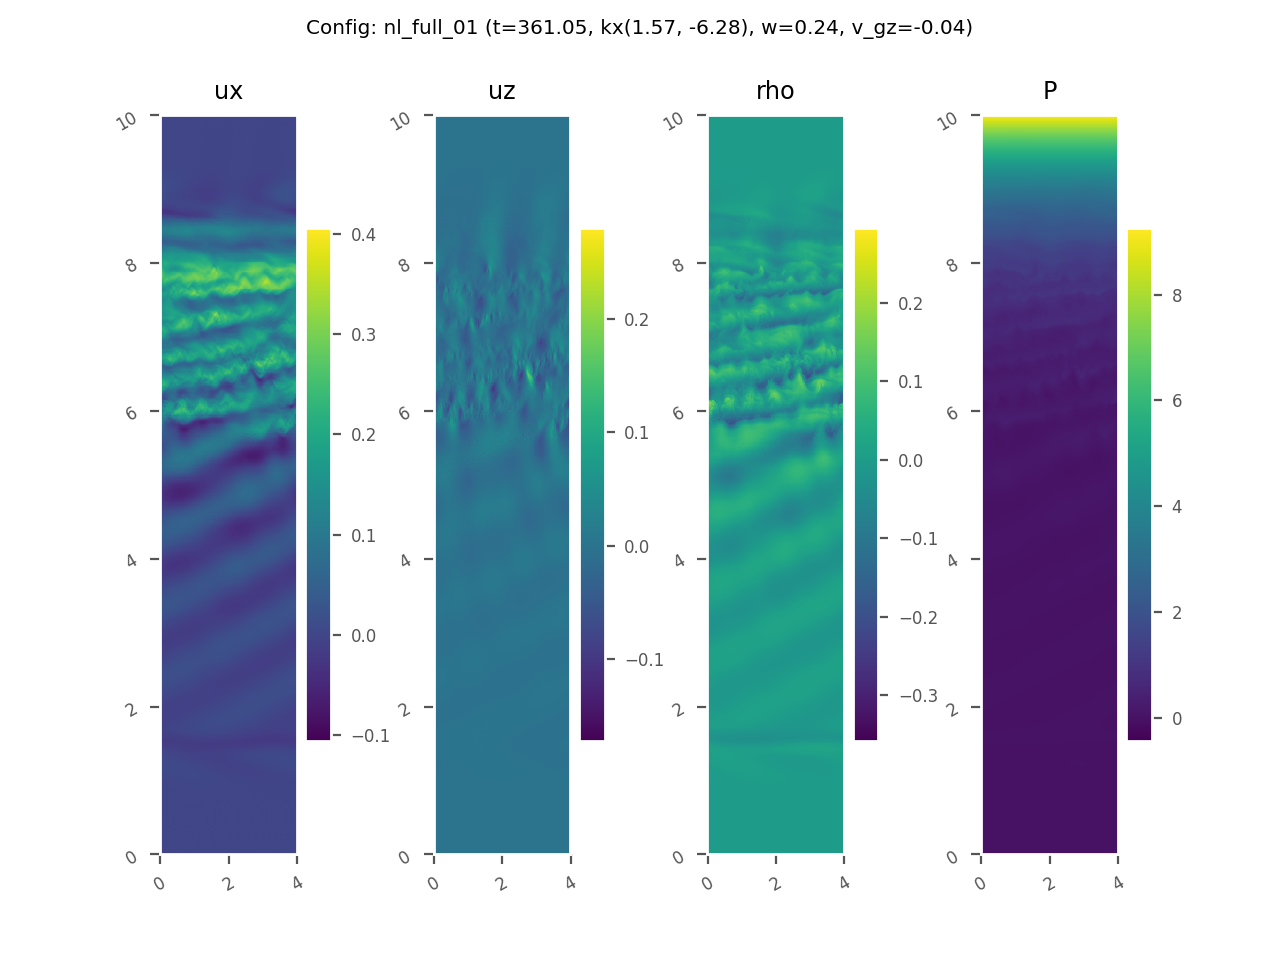
\includegraphics[width=0.5\textwidth]{plots/nl_full_01.png}
    \caption{Low viscosity simulation showing seemingly KHI-like
    features.}\label{fig:nl_full_01}
\end{figure}

This seems to suggest that our reference simulation is viscosity limited. This
is perhaps physical: a Richardson number $\sim 0.25$ incurs the KHI which saps
energy and angular momentum from the flow. It is conceivable then that our
numerical viscosity is physically motivated as a effective KHI viscosity.

\section{Boussinesq Local Simulation (Speculative)}\label{s:bouss}

Alternatively, we can attempt direct numerical simulation probing lower
Richardson numbers. We will move to the Boussinesq approximation and set up a
mean flow as an initial condition. This relaxes the constraint that the domain
must be sufficiently large to permit substantial $e^{z/H}$ growth of the mean
flow $\bar{U}_0$ and allows us to probe much finer vertical resolution.

The physical equations in the Boussinesq approximation are:
\begin{subequations}\label{se:bouss}
    \begin{align}
        \vec{\nabla} \cdot \vec{u} &= 0,\\
        \pd{\rho_1}{t} + \p*{\vec{u} \cdot \vec{\nabla}}\rho_1
            - N^2\frac{\rho_0 u_z}{g} &= 0,\\
        \pd{\vec{u}}{t} + \p*{\vec{u} \cdot \vec{\nabla}}\vec{u}
            + \frac{\vec{\nabla}P_1}{\rho_0}
            + \frac{\rho_1 g\hat{z}}{\rho_0} &= 0.
    \end{align}
\end{subequations}
In these equations, we take $\rho_0(z) = \rho_0 = 1$ a constant reference
density. We nondimensionalize $\rho_0 = N = g = 1$. By using a subgrid model
(details \autoref{ss:bouss_impl}), we are able to probe significantly smaller
Richardson numbers.

\subsection{Low-Resolution Simulation}

The parameters of the simulation differ slightly; since we do not have
exponential density stratification to induce $\bar{U}_0 \propto e^{z/H}$ growth,
we initialize the system with an initial $\bar{U}_0(z) \leq \bar{U}_c$,
simulating a later phase of the stratified simulation where the critical layer
has propagated deep into the domain.

Sample snapshots from a reference simulation are \autoref{fig:bouss_1}.
\begin{figure}[h]
    \centering
    \begin{subfigure}{0.5\textwidth}
        \centering
        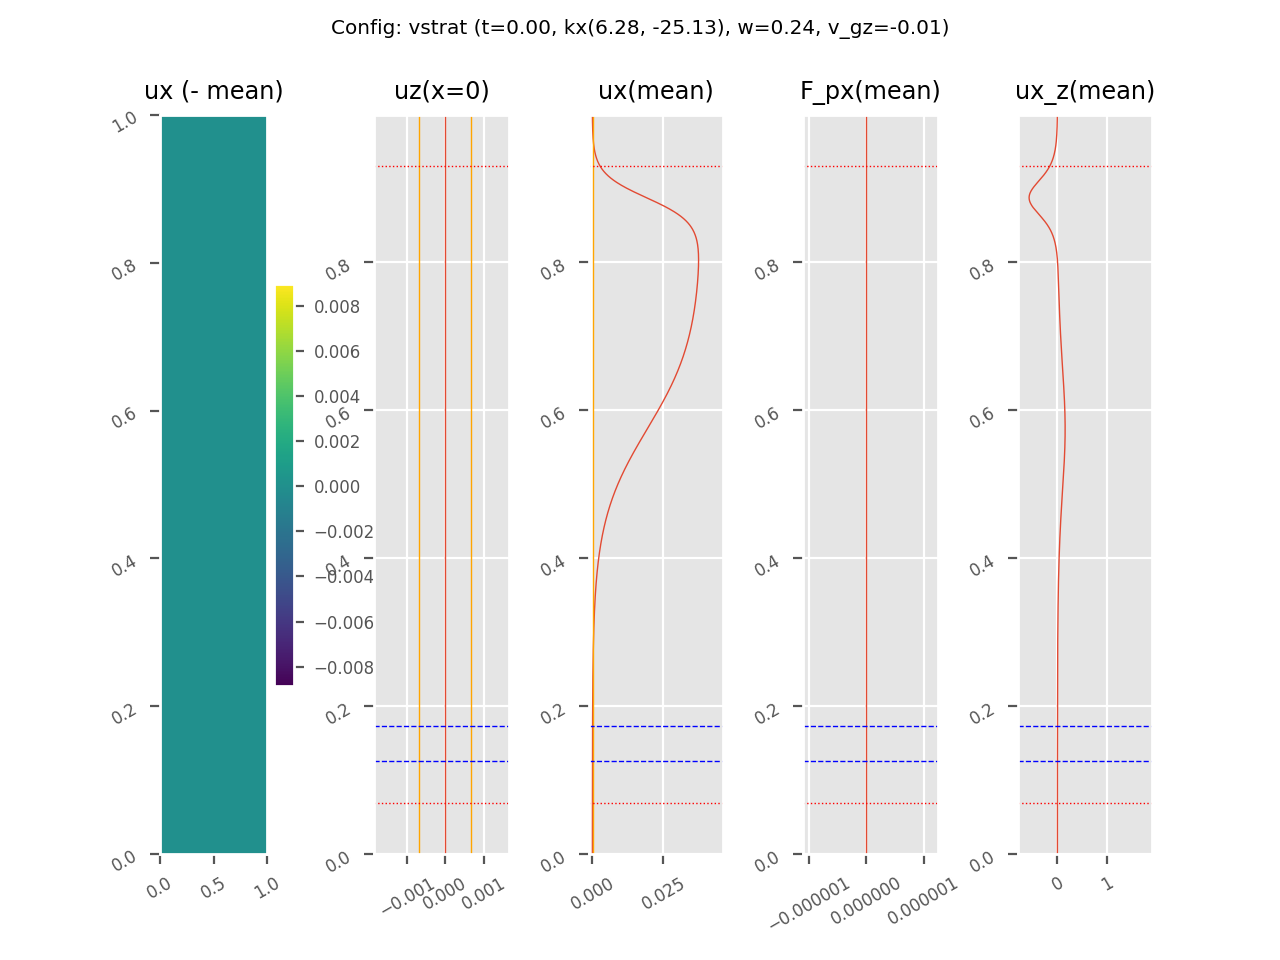
\includegraphics[width=\textwidth]{plots/vstrat_1.png}
        \caption{Boussinesq simulation initial condition.}
    \end{subfigure}

    \begin{subfigure}{0.5\textwidth}
        \centering
        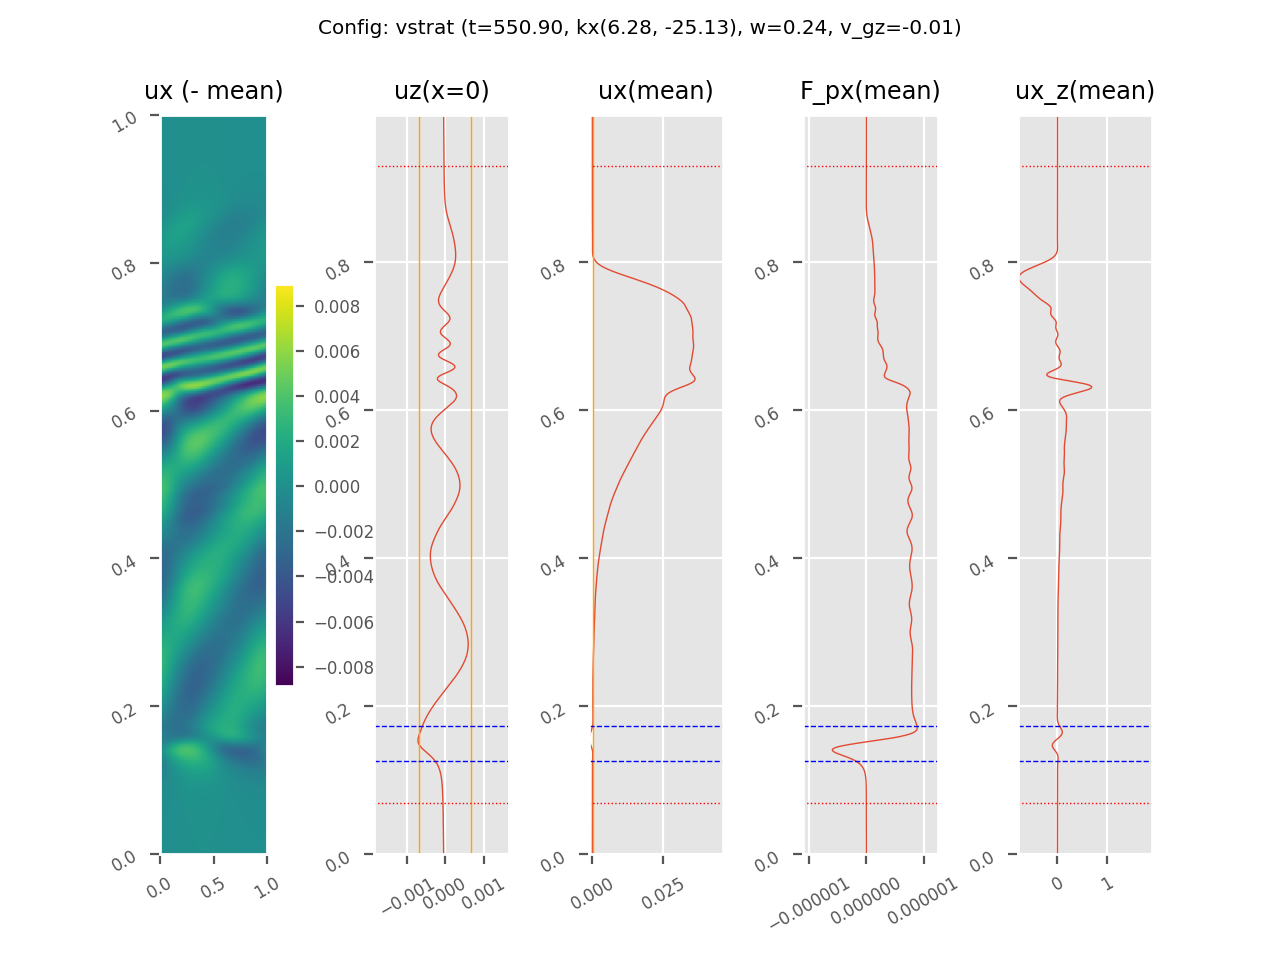
\includegraphics[width=\textwidth]{plots/vstrat_2.png}
        \caption{At later time, when critical layer absorption has begun.}
    \end{subfigure}

    \begin{subfigure}{0.5\textwidth}
        \centering
        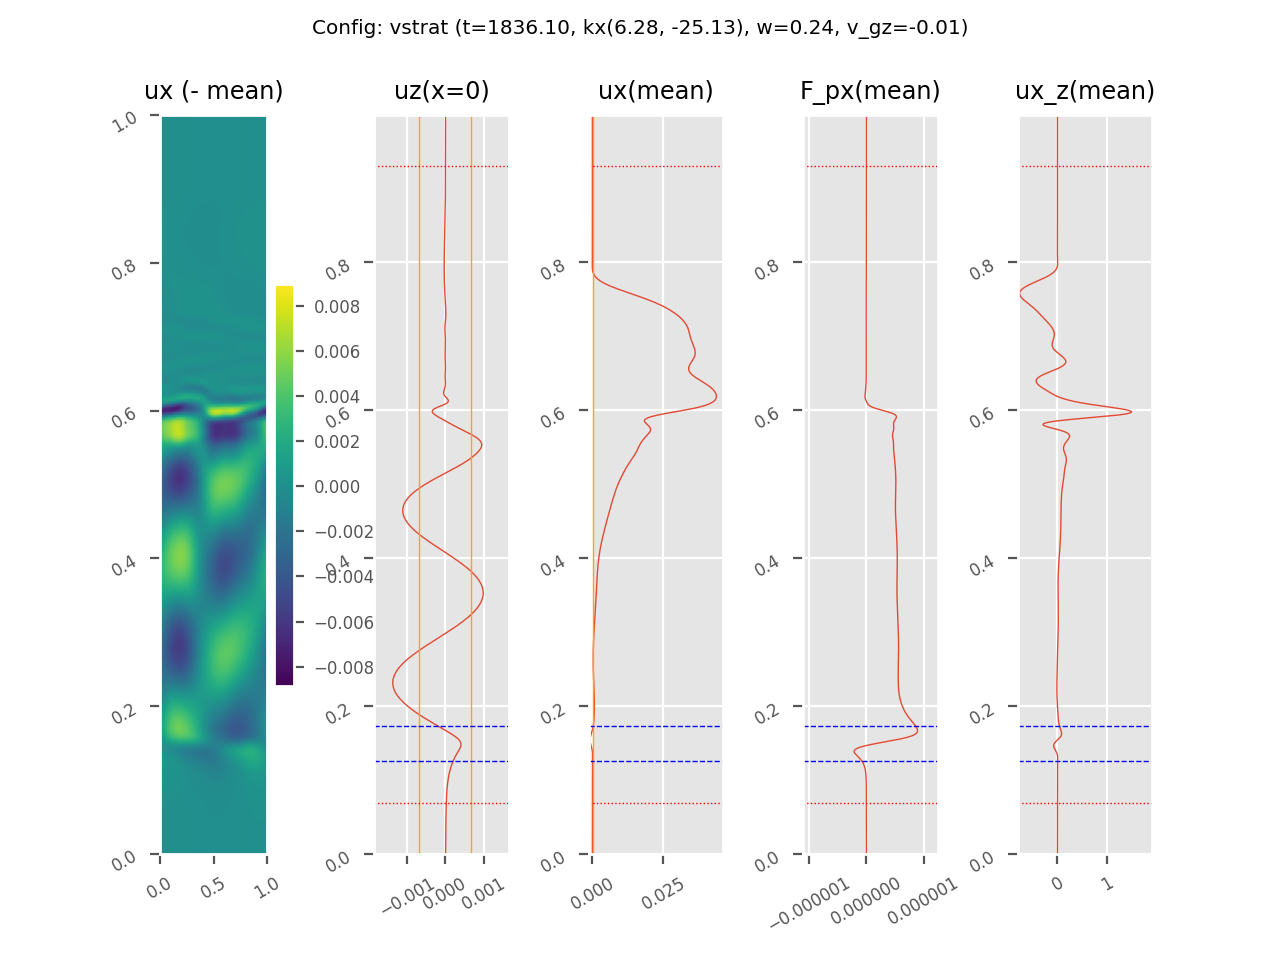
\includegraphics[width=\textwidth]{plots/vstrat_3.png}
        \caption{At an even later time, a strong reflective character seems to
        emerge as the Richardson number $\to 0.5$.}
    \end{subfigure}
    \caption{Boussinesq simulation snapshots.}\label{fig:bouss_1}
\end{figure}
The resulting front velocity and Richardson number are depicted in
\autoref{fig:bouss}. Most important to note are the significantly diminished
critical layer velocity compared to the prediction (owing to critical layer
reflection) and the Richardson number which approaches the critical $1/4$ value
for KHI-instability.
\begin{figure}[t]
    \centering
    \begin{subfigure}{0.5\textwidth}
        \centering
        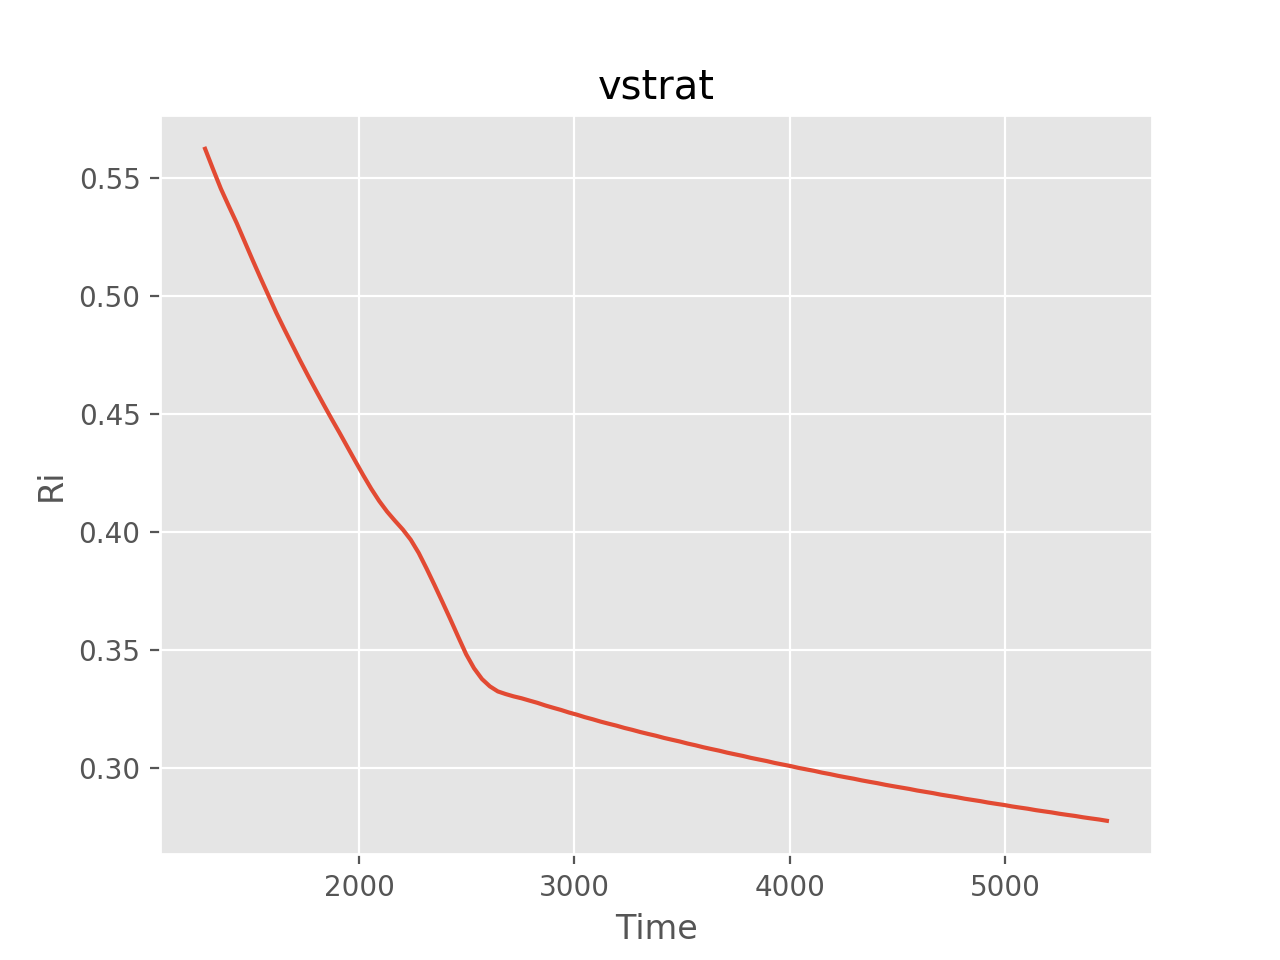
\includegraphics[width=\textwidth]{plots/vstrat_ri.png}
        \caption{Richardson number evolution over time.}
    \end{subfigure}

    \begin{subfigure}{0.5\textwidth}
        \centering
        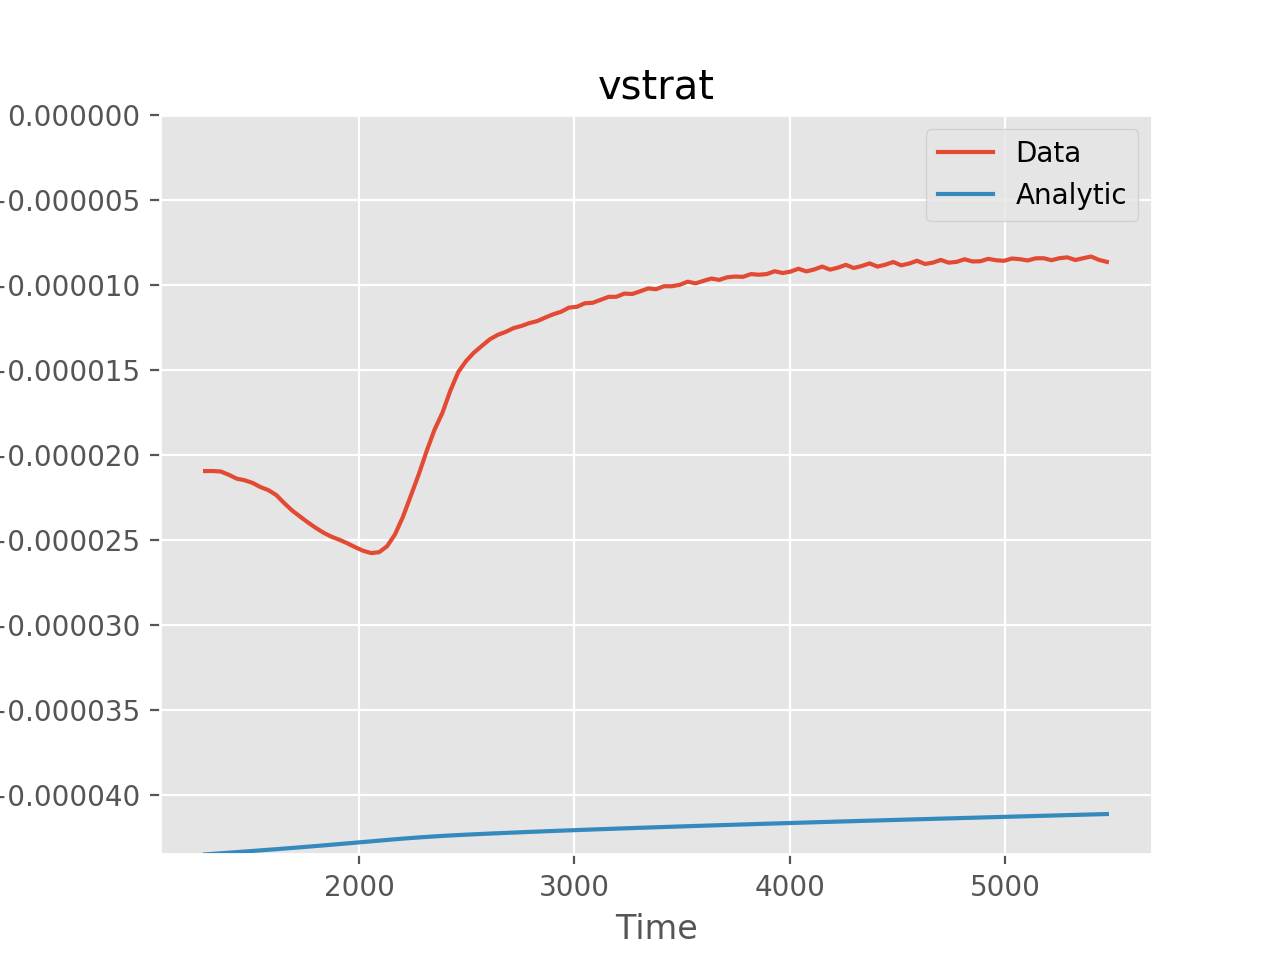
\includegraphics[width=\textwidth]{plots/vstrat_front_v.png}
        \caption{Front velocity compared to analytical \autoref{eq:u0_lin}
        prediction.}
    \end{subfigure}
    \caption{Boussinesq data analysis plots.}\label{fig:bouss}
\end{figure}

YUBONOTE\@: The next step would be to run simulations at sufficient resolution to
resolve the KHI (only possible in the Boussinesq system, where we are not
required to have a sufficiently large vertical domain to capture exponential
growth and can choose ever smaller vertical domains); I have started to try this
but haven't resolved the resultant numerical issues yet.

\clearpage
\onecolumngrid
\appendix

\section{Equation Implementations}

We denote $x \in [0, L_x], z \in [0, L_z]$ the simulation domain and $N_x, N_z$
the number of spectral modes in the respective dimensions.

\subsection{Stratified Fluid}\label{ss:strat_impl}

We introduce variable $T = P/\rho$. We then mandate $\rho_0, T_0$ background
fields satisfy hydrostatic equilibrium $\vec{\nabla}T_0 + T_0 \vec{\nabla}\rho_0
+ \vec{g} = 0$. Taking isothermal stratification, we find $T_0 = gH$. Making
then substitution of variables $\Upsilon = \ln \rho - \ln \rho_0$ and $T_1 = T -
T_0$ deviations from the background state, the exact fluid equations in the new
variables are:
\begin{subequations}\label{se:fc_var}
    \begin{align}
        \vec{\nabla} \cdot \vec{u} &= 0,\\
        \pd{\Upsilon}{t} - \frac{u_z}{H} &= 0,\\
        \pd{u_x}{t} + \p*{\vec{u} \cdot \vec{\nabla}}u_x
            + \pd{T}{x} + gH\pd{\Upsilon}{x}
            + T_1 \pd{\Upsilon}{x} &= 0,\\
        \pd{u_z}{t} + \p*{\vec{u} \cdot \vec{\nabla}}u_z
            + \pd{T}{z} + gH\pd{\Upsilon}{z}
            + T_1 \pd{\Upsilon}{z} - \frac{T_1}{H} &= 0.
    \end{align}
\end{subequations}

These are implemented as:
\begin{subequations}\label{se:curr_num}
    \begin{align}
        \vec{\nabla} \cdot \vec{u} &= 0,\\
        \pd{\Upsilon}{t} - \frac{u_z}{H}
            - \nu \nabla^2 \Upsilon &= -\Gamma(z) \Upsilon
                - \p*{\vec{u} \cdot \vec{\nabla}}\Upsilon
                + \frac{F}{\rho_0(z)}e^{-\frac{(z - z_0)^2}{2\sigma^2}}
                    \cos \p*{k_xx - \omega t},\\
        \pd{u_x}{t} + \pd{T}{x} + gH\pd{\Upsilon}{x}
            - \nu \nabla^2 u_x
            &= -\Gamma(z) u_x
                - \p*{\vec{u} \cdot \vec{\nabla}}u_x
                - T_1 \pd{\Upsilon}{x},\\
        \pd{u_z}{t} + \pd{T}{z} + gH\pd{\Upsilon}{z} - \frac{T_1}{H}
            - \nu \nabla^2 u_z &= -\Gamma(z) u_z
                - \p*{\vec{u} \cdot \vec{\nabla}}u_z
                - T_1 \pd{\Upsilon}{z},\\
    \Gamma(z) &= 7.5\s*{2 + \tanh \frac{z - z_T}{(L_z - z_T) / 2}
        + \tanh \frac{z_B - z}{z_B / 2}},\label{eq:Gamma}
    \end{align}
\end{subequations}
where $z_B = 0.05L_z, z_T = 0.95L_z$ are the boundaries of the damping zones. A
Navier-Stokes numerical viscosity $\nu$ is used to damp high wavenumbers and
regularize the nonlinear cascade at near grid resolution: $\nu \sim 0.2
\frac{\omega}{\abs*{k_z}}\frac{L_z}{2\pi N_z}$ was found to be suitable for $N_z
= 1024$, where $k_z$ is the wavenumber of the excited linear mode.

\subsection{Boussinesq Fluid}\label{ss:bouss_impl}

In the Boussinesq system, there is no need to transform to $T, \Upsilon$
variables as $\rho_0$ is constant. Including numerical terms and driving terms,
our full equations are
\begin{subequations}\label{se:bouss_num}
    \begin{align}
        \vec{\nabla} \cdot \vec{u}_1 &= 0,\\
        \pd{\rho_1}{t} - \frac{\rho_0 u_z}{H}
            - \nu \nabla^6 \rho_1
            &= -\Gamma(z) \rho_1
                - \p*{\vec{u} \cdot \vec{\nabla}}\rho_1
                + Fe^{-\frac{(z - z_0)^2}{2\sigma^2}}
                    \cos \p*{k_xx - \omega t},\\
        \pd{u_x}{t} + \frac{\partial_x P}{\rho_0}
            - \nu \nabla^6 u_x
            &= -\Gamma(z) u_x
                - \p*{\vec{u} \cdot \vec{\nabla}}u_x,\\
        \pd{u_z}{t} + \frac{\partial_z P}{\rho_0}
            + \frac{\rho_1 g}{\rho_0}
            - \nu \nabla^6 u_z
            &= -\Gamma(z) u_z
                - \p*{\vec{u} \cdot \vec{\nabla}}u_z.
    \end{align}
\end{subequations}
$\Gamma(z)$ is as \autoref{eq:Gamma}. We use subgrid model $\nabla^6$ (cite) to
decrease the effect of viscosity on scales above the grid resolution.

\end{document}

